\section{Introduction}
\label{sec:intro}

Please see advice from \href{https://www.cs.columbia.edu/~hgs/etc/intro-style.html}{Prof. Kurose} on how to write a good introduction. 


\textit{A good paper introduction is fairly formulaic. If you follow a simple set of rules, you can write a very good introduction. The following outline can be varied. For example, you can use two paragraphs instead of one, or you can place more emphasis on one aspect of the intro than another. But in all cases, all of the points below need to be covered in an introduction, and in most papers, you don't need to cover anything more in an introduction.}

\textbf{Paragraph 1: Motivation.} \textit{At a high level, what is the problem area you are working in and why is it important? It is important to set the larger context here. Why is the problem of interest and importance to the larger community?}

\textbf{Paragraph 2}: \textit{What is the specific problem considered in this paper? This paragraph narrows down the topic area of the paper. In the first paragraph you have established general context and importance. Here you establish specific context and background.}

\textbf{Paragraph 3}: \textit{"In this paper, we show that ...". This is the key paragraph in the intro - you summarize, in one paragraph, what are the main contributions of your paper given the context you have established in paragraphs 1 and 2. What is the general approach taken? Why are the specific results significant? This paragraph must be really really good. If you can't "sell" your work at a high level in a paragraph in the intro, then you are in trouble. As a reader or reviewer, this is the paragraph that I always look for, and read very carefully.
You should think about how to structure this one or two paragraph summary of what your paper is all about. If there are two or three main results, then you might consider itemizing them with bullets or in test (e.g., "First, ..."). If the results fall broadly into two categories, you can bring out that distinction here. For example, "Our results are both theoretical and applied in nature. (two sentences follow, one each on theory and application)"}

\textbf{Paragraph 4}: \textit{At a high level what are the differences in what you are doing, and what others have done? Keep this at a high level, you can refer to a future section where specific details and differences will be given. But it is important for the reader to know at a high level, what is new about this work compared to other work in the area.}

\textbf{Paragraph 5}: \textit{"The remainder of this paper is structured as follows..." Give the reader a roadmap for the rest of the paper. Avoid redundant phrasing, "In Section 2, In section 3, ... In Section 4, ... " etc.}

\textbf{Paragraph 1}: \hl{"The rapid expansion of internet applications has made network traffic classification a critical task for efficient network management. Accurately identifying traffic types enables network operators to allocate resources effectively, improve user experiences, and optimize operational costs. As encrypted traffic and specialized applications like online gaming and music streaming become increasingly prevalent, traditional classification methods struggle to keep pace. Addressing these challenges is vital for both academic research and practical deployment."}

\textbf{Paragraph 2}: \hl{"While general traffic classification has been extensively studied, distinguishing between domain-specific types of traffic—such as gaming and music—remains an open problem. These traffic types exhibit unique patterns and requirements, such as low latency for gaming or high throughput for music streaming, which are not captured by existing datasets or classification models. Current approaches fail to leverage tailored datasets or advanced machine learning techniques to address these distinctions, leaving a gap in both research and application."}

\textbf{Paragraph 3}: \hl{"In this paper, we address the challenge of domain-specific traffic classification through machine learning, focusing on distinguishing between gaming and music traffic. Our key contributions include: 
- Custom Dataset Creation: Leveraging the NetUnicorn framework, we collect tailored traffic data specific to gaming and music applications.
- Feature Engineering and Model Evaluation: We extract packet-level features, including size, frequency, and flow duration, and evaluate various machine learning models to identify the most effective classifier for this problem.
- Insights and Impact: Our work demonstrates the feasibility of accurately classifying gaming and music traffic, even with limited labeled data, and highlights the potential for fine-grained traffic optimization."}

\textbf{Paragraph 4}: \hl{"Unlike previous studies that focus on broader traffic categories, our approach emphasizes domain-specific classification, a level of granularity often overlooked in traditional methods. Additionally, while most studies rely heavily on existing datasets, our work introduces a custom data collection methodology and explores the specific behaviors of gaming and music traffic, addressing a significant gap in the field."}

\textbf{Paragraph 5}: \hl{"The remainder of this paper is structured as follows. Section 2 reviews related work and highlights gaps in current methodologies. Section 3 describes our data collection process and feature extraction pipeline. Section 4 details the machine learning models used and their evaluation. In Section 5, we present results and discuss their implications. Finally, Section 6 concludes the paper and outlines future research directions."}

A few general tips:
\begin{itemize}
    \item Don't spend a lot of time into the introduction telling the reader about what you don't do in the paper. Be clear about what you do do, but don't dwell here on what you don't do.
    \item Does each paragraph have a theme sentence that sets the stage for the entire paragraph? Are the sentences and topics in the paragraph all related to each other?
    \item Do all of your tenses match up in a paragraph?
\end{itemize}


Here is a checklist for a good intro from \href{https://docs.google.com/document/d/14g-4txTMwJ4YL61qOcaH6bJWKh59PkI1S-FB1KjeMS4/edit}{Prof. Sherry}: 
\begin{itemize}
    \item Clearly identifies and discusses research problem statement
    \item Motivation and benefits of the research are identified and discussed completely.
    \item Solution/insights of the research are well-articulated.
    \item The problem and/or solution is novel: no one has published something similar before.
    \item ``Teaser'' results provide a useful summary of ``key results''/conclusions of the work.
\end{itemize}


\begin{figure}[t] 
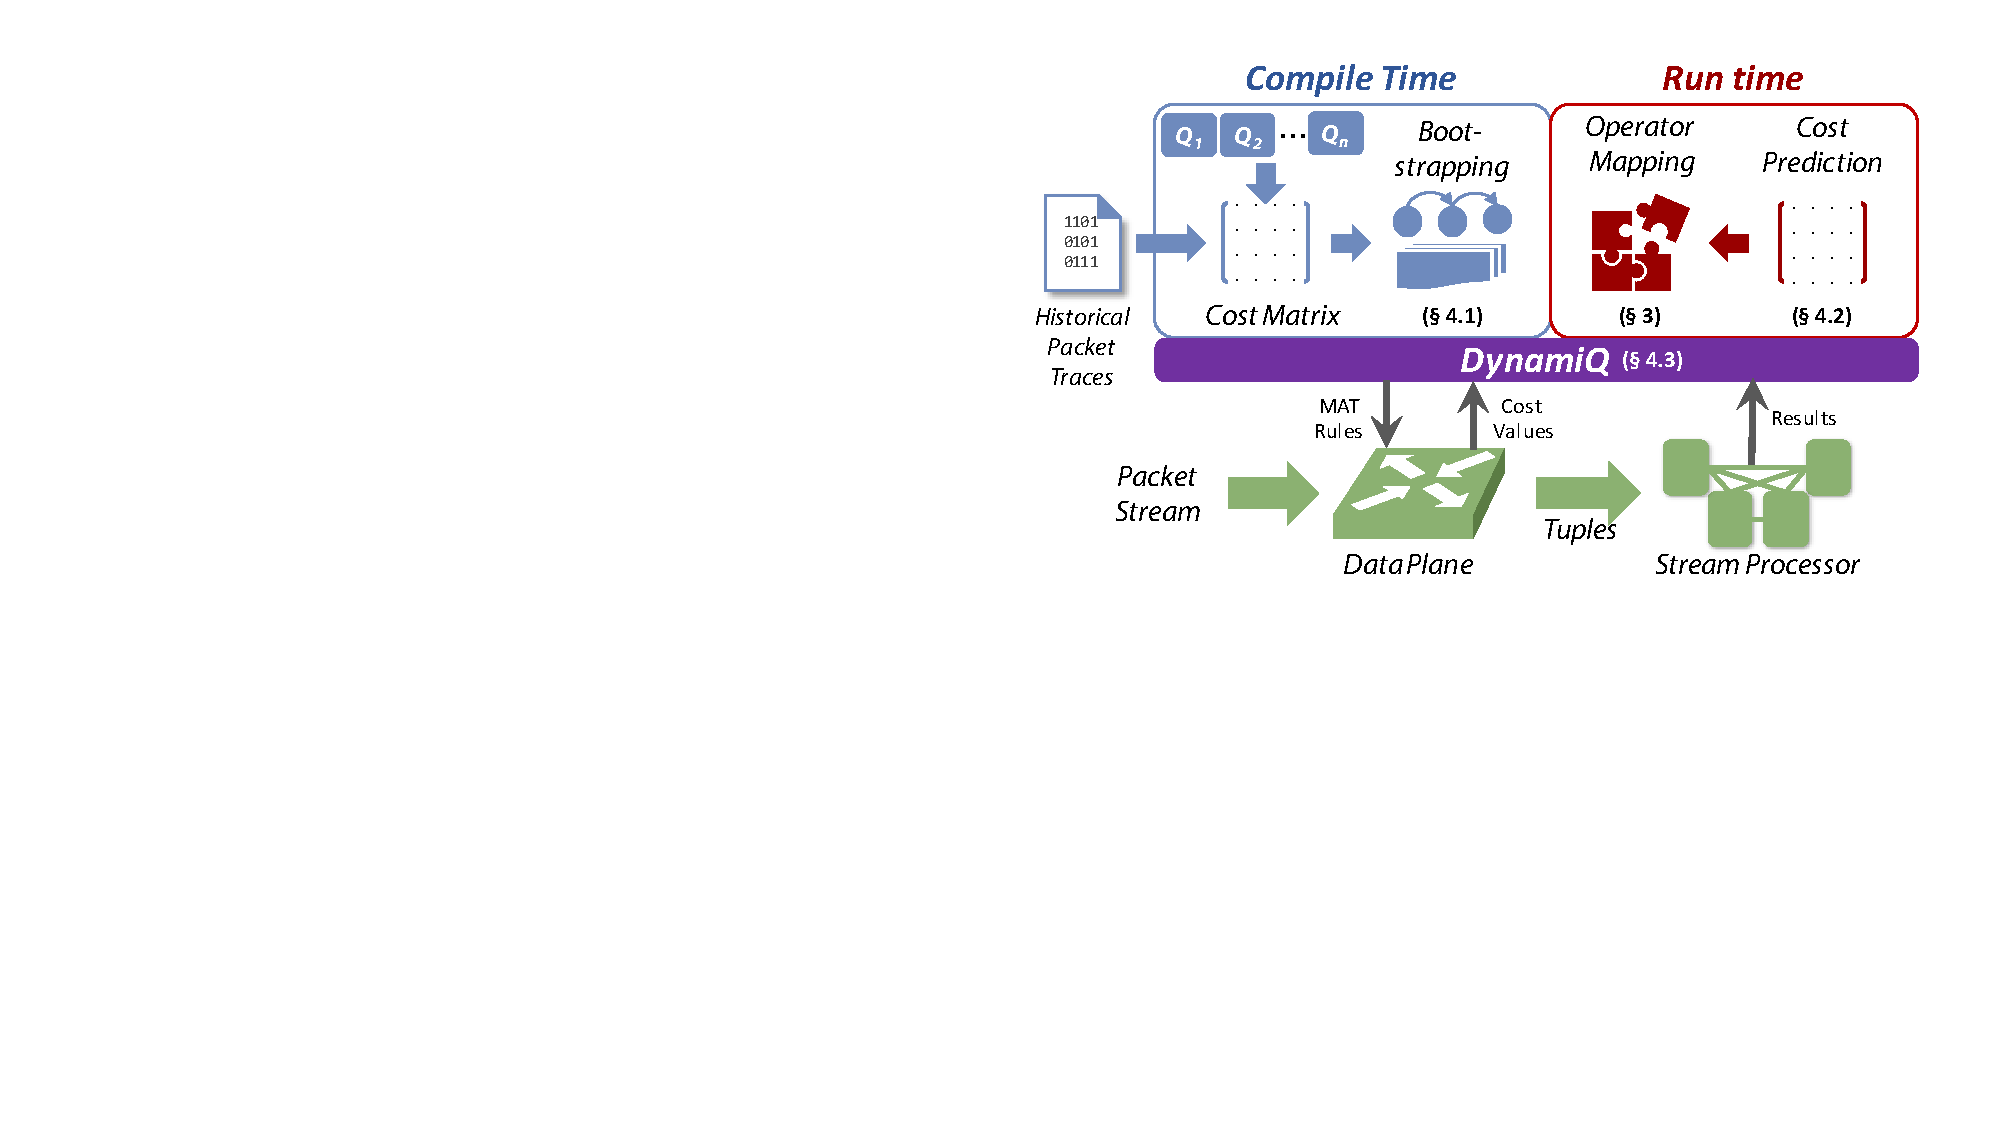
\includegraphics[width=\linewidth]{dynamiq-nutshell.pdf}
\caption{{Sample figure~\cite{sonata}} \label{fig:dynamiq-nutshell}
}
\vspace{-.15in}
\end{figure}
